\section{Программное обеспечение системы компьютерного зрения в антропометрии}
Приложение создано для обработки видео на смартфонах, оно основано на алгоритмах компьютерного зрения в антропометрии с использованием поддержки среды Android и библиотек OpenCV, Min3D, MakeHuman. В данной диссертации применяется система компьютерного зрения в антропометрии для создания приложений в областях пошива одежды (E-Tailor) и фитнеса (E-Fitness). Приложения загружены на онлайн-магазин GooglePlay и их можно скачать бесплатно. Системные требования: версия Android от 4.4.2, передняя камера с разрешением 2.0 мп или выше.

После загрузки и установки, система автоматически загрузит и установит библиотеку OpenCV для телефона.

\subsection{Применение системы компьютерного зрения в антропометрии для пошива одежды (E-Tailor)}
Программа <<E-Taloir>> предназначена для пошива одежды.
При запуске программы появляется главное окно формы \ref{img42}

\begin{itemize}
\item <<Measure Me>> В рабочей области отображается видеопоследовательность, область обнаружения объектов и извлечение антропометрических признаков;
\item <<Credit>> Контакты с командой разработчиков;
\item <<Exit>> Позволяет осуществить выход из программы.
\end{itemize}

\begin{figure}[ht!]
\centering
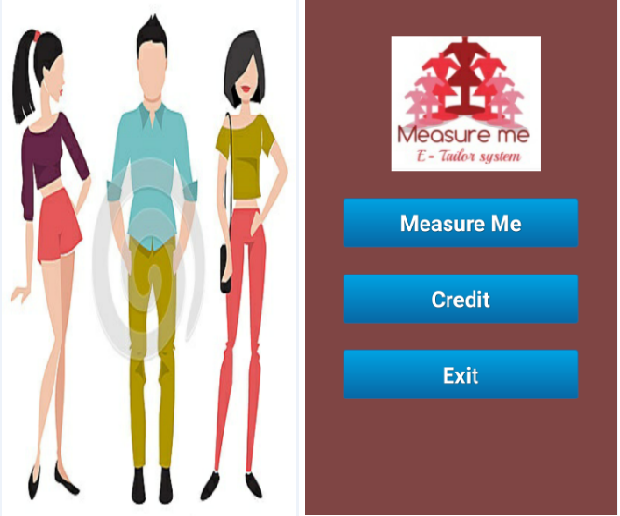
\includegraphics [scale=0.5] {images/h42.png}
\begin{center}
%\captionsetup{justification=justified, labelsep=period}
\caption{Основный интерфейс приложения E-Tailor} \label{img42}
\end{center}
\end{figure}
\textbf{Основные функции приложения E-Tailor \ref{img43}}

\begin{itemize}
	\item Позволять пользователям добавлять информацию;
	\item Показать 3D-модель на основе антропометрических признаков и классификации данных;
	\item Позволять пользователям выбрать марки одежды и классифицировать размеры одежды.
\end{itemize}

\begin{figure}[ht!]
\centering
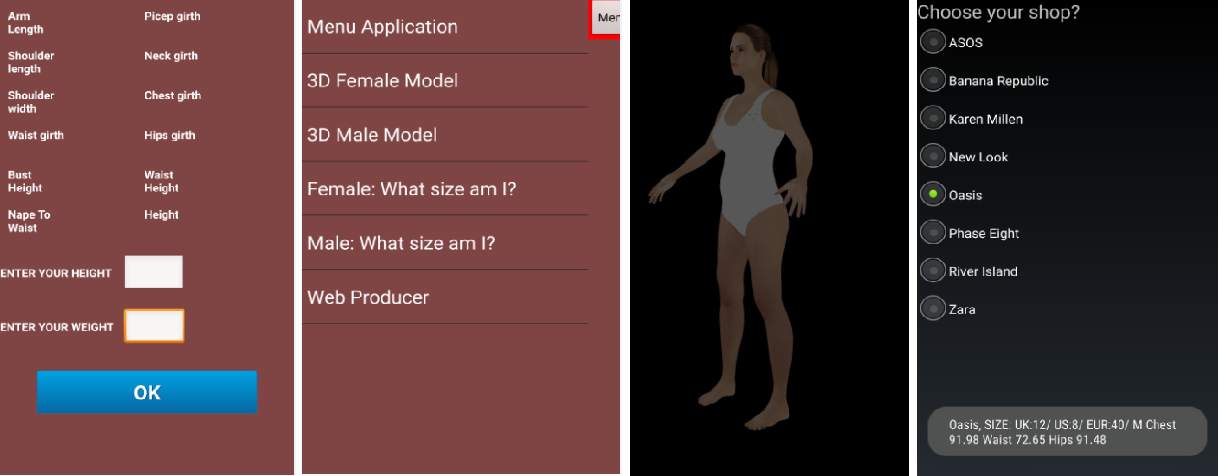
\includegraphics [scale=0.5] {images/h43.png}
\begin{center}
%\captionsetup{justification=justified, labelsep=period}
\caption{Результат функции выбора размеров одежды} \label{img43}
\end{center}
\end{figure}


%-------------------------
\subsection{Применение системы компьютерного зрения в антропометрии для фитнеса (E-Fitness)}
Программа <<E-Fitness>> предназначена для фитнеса.
При запуске программы появляется главное окно формы \ref{img38}

\begin{itemize}
\item <<Measure Me>> В рабочей области отображается видеопоследовательность, область обнаружения объектов и извлечение антропометрических признаков;
\item <<Credit>> Контакты с командой разработчиков;
\item <<Exit>> Позволяет осуществить выход из программы.
\end{itemize}

\begin{figure}[ht!]
\centering
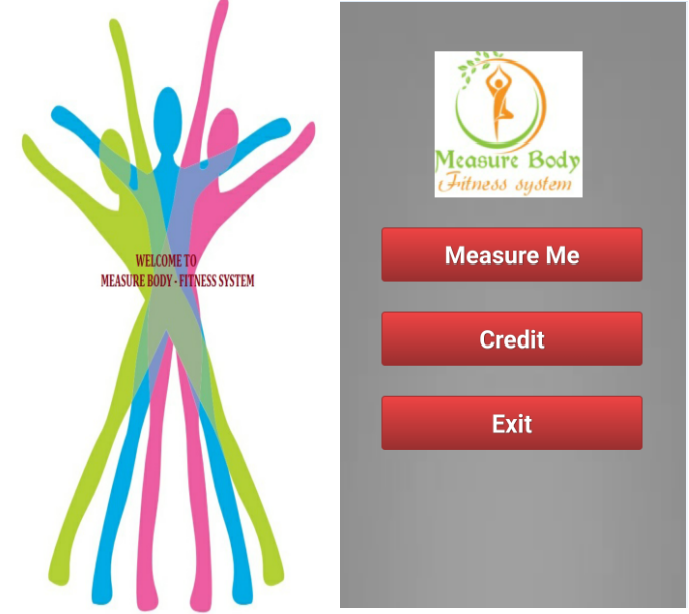
\includegraphics [scale=0.5] {images/h38.png}
\begin{center}
%\captionsetup{justification=justified, labelsep=period}
\caption{Основный интерфейс приложения E-Fitness} \label{img38}
\end{center}
\end{figure}

\textbf{Основные функции приложения E-Fitness}\ref{img39}

\begin{itemize}
	\item Позволять пользователям добавлять информацию;
	\item Показать 3D-модель на основе антропометрических признаков и классификации данных \ref{img40};
	\item Анализ антропометрических признаков на основе стандартов Fitness \ref{img41}.
\end{itemize}

\begin{figure}[ht!]
\centering
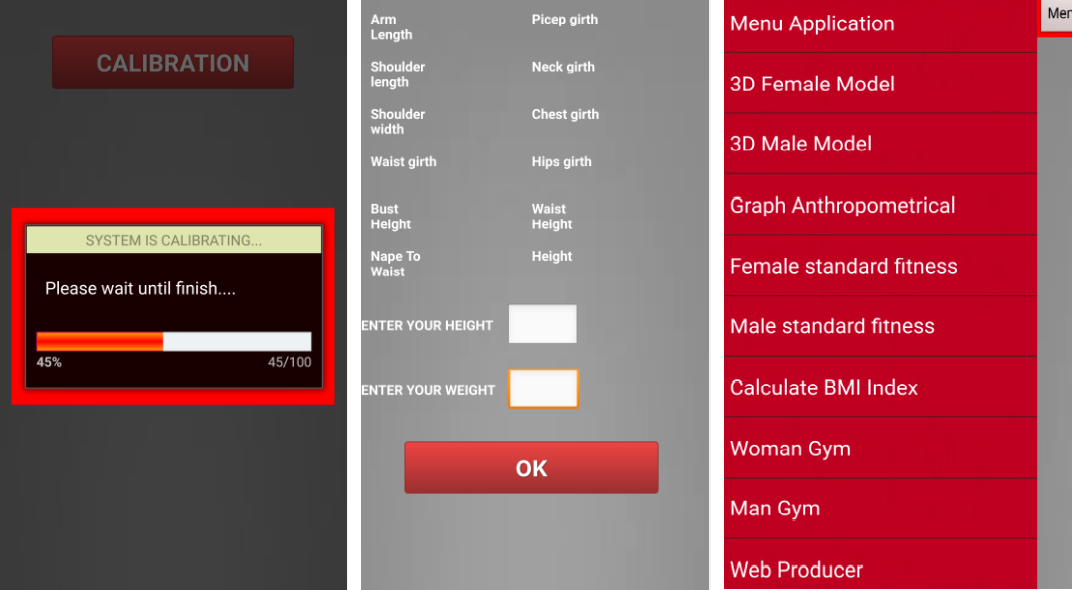
\includegraphics [scale=0.5] {images/h39.png}
\begin{center}
%\captionsetup{justification=justified, labelsep=period}
\caption{Интерфейс работы программы } \label{img39}
\end{center}
\end{figure}

\begin{figure}[ht!]
\centering
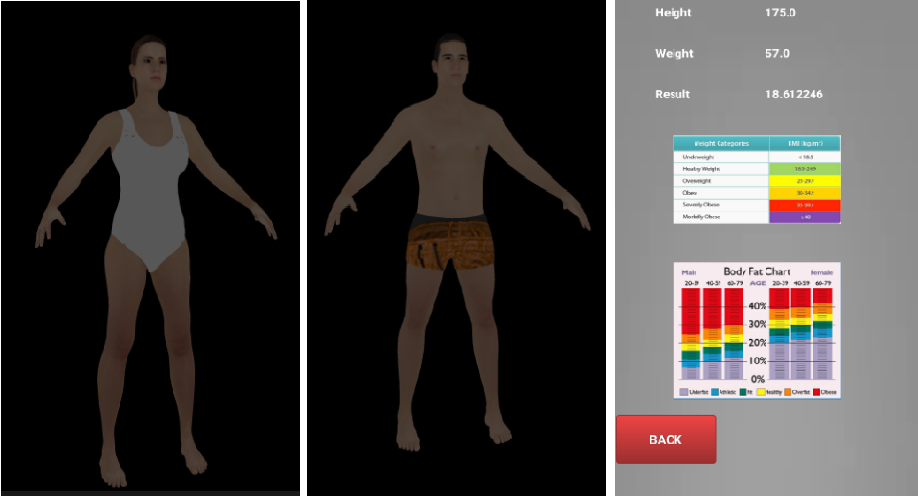
\includegraphics [scale=0.5] {images/h40.png}
\begin{center}
%\captionsetup{justification=justified, labelsep=period}
\caption{Результат 3D-моделей} \label{img40}
\end{center}
\end{figure}
В (рис.\ref{img41}) описывает анализ антропометрических признаков по фитнес-стандартам. Где красная линия - реальные размеры, зеленная линия - размеры по фитнес-стандартам. Приложение позволяет пользователям сравнить свои параметры с размерами по фитнес-стандартам.  
\begin{figure}[ht!]
\centering
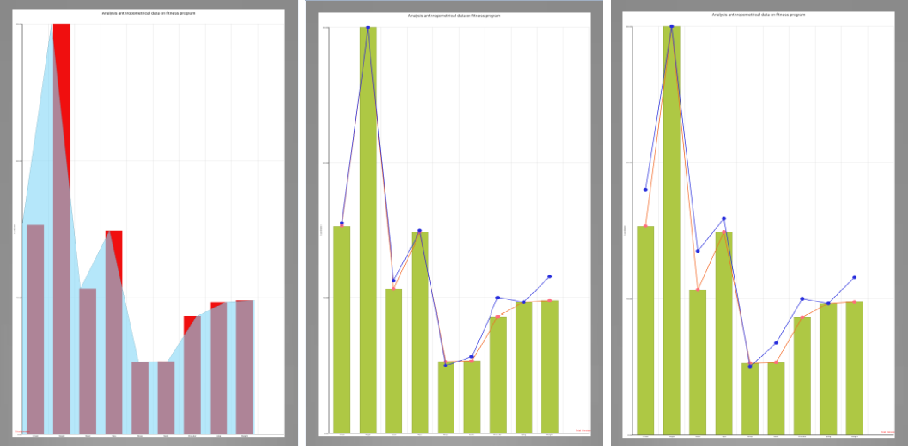
\includegraphics [scale=0.5] {images/h41.png}
\begin{center}
%\captionsetup{justification=justified, labelsep=period}
\caption{Результат анализа антропометрических признаков на основе стандартам Fitness} \label{img41}
\end{center}
\end{figure}
%-------------------------